\begin{problem}
  Suppose two cameras fixate on a point P (see Figure \ref{fig:1}) in space such that
  their optical axes intersect at that point.
  Show that if the image coordinates are normalized so that the
  coordinate system origin $(0, 0)$ coincides with the principal point,
  the $\bF_{33}$ element of the fundamental matrix $\bF$ is zero.

  \begin{figure}[H]
    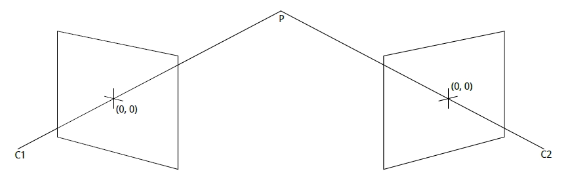
\includegraphics[width=0.7\textwidth]{figures/rectified-pair}
    \caption{$C_1$ and $C_2$ are the optical centers.  The principal axes intersect at point $P$.}
    ~\label{fig:1}
  \end{figure}
\end{problem}

\begin{answer}



  
  The fundamental matrix $\bF$ is given by
  \[
    \bF = (\bK')^{-\top} [\bT]_\times \bR \bK^{-1},
  \]
  where $\bK$ and $\bK'$ are the intrinsic matrices of the two cameras,
  $\bT$ is the translation vector from $C_1$ to $C_2$, and $\bR$ is the rotation matrix
  from $C_1$ to $C_2$.
  Two points $\bx$ and $\bx'$ in the two images are related by $\bx'^\top \bF \bx = \bzero$.
  When the image coordinates are normalized so that the
  coordinate system origin $(0, 0)$ coincides with the principal point,
  we have $\bx = \bmat{0 & 0 & 1}^\top$ and $\bx' = \bmat{0 & 0 & 1}^\top$,
  which implies that
  
  \begin{align*}
    \bmat{0 & 0 & 1} \bF \bmat{0 \\ 0 \\ 1} &= \bzero \\
    \bmat{0 & 0 & 1}
      \bmat{\bF_{11} & \bF_{12} & \bF_{13} \\
            \bF_{21} & \bF_{22} & \bF_{23} \\
            \bF_{31} & \bF_{32} & \bF_{33}}
    \bmat{0 \\ 0 \\ 1} &= \bzero \\
    \bmat{0 & 0 & 1} \bmat{\bF_{13} \\ \bF_{23} \\ \bF_{33}} &= \bzero \\
    \bF_{33} &= \bzero.
  \end{align*}
\end{answer}
